\chapter{OpenGL}
\todo{This Chapter describes OpenGL and which of its functionalities we have used to create our game.}

\section{Analysis}
OpenGL is a 2D and 3D graphics API. It is cross-platform API that specifies a standard for 3D graphics processing hardware. The newest version of OpenGL is $4.3$ which was released August 2012. Android have support for \ac{opengles} up to version $2.0$. \ac{opengles} $1.1$ is based on the OpenGL $1.5$ specification and is fully backwards compatible with $1.0$, and \ac{opengles} $2.0$ is based on OpenGL $2.0$. Android $1.0$ and later versions have support for \ac{opengles} $1.0$ and $1.1$ specifications. Android $2.2$ added support for \ac{opengles} $2.0$. \citep{androidopengl, khronosopengl, khronosopengles}

\subsection*{Choice of \ac{opengles} Version}
When using \ac{opengles} on the Android platform, the default \ac{opengles} version is $1.x$. If you want to use version $2.0$ you need to explicitly write that you are using it. Version $2.0$ should have better performance and more possibilities than the older version, but the Android developers guide says:
\begin{quote}
\textit{"Developers who are new to OpenGL may find coding for \ac{opengles} $1.0$/$1.1$ faster and more convenient."} \citep{androidopengl}
\end{quote}
Since we are newbies to OpenGL we have chosen version $1.x$. One big difference between $1.x$ and $2.0$ is that you have to write your own shaders in versions $2.0$, this allows for easier effects customisation. The Train game does not really require much special effects other than simple drawing of textures.

\section{Design}
Firstly \ref{fig:terminology} shows how we represent abstract class names and how we denote public or private attributes and methods. A minus denotes a private attribute/method, and a plus denotes a public attribute/method. Italic class names are abstract classes. \todo{Skal det stå her? Det må være C\# UML standard det her.}
\begin{figure}[H]
\centering
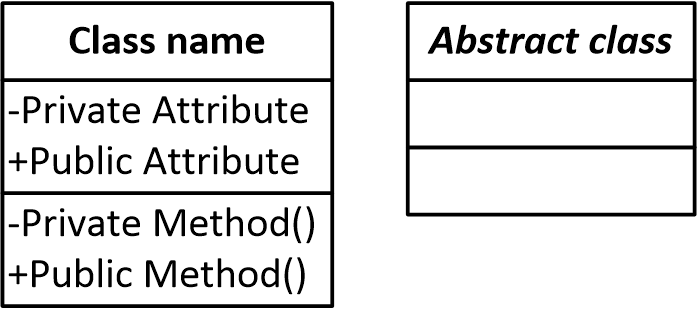
\includegraphics[width=0.4\linewidth]{img/terminology.png}
\caption{The way we make UML described in a figure.}
\label{fig:terminology}
\end{figure}
Thinking about what the game is suppose to do we came up with the different objects we need to be able to render. We needed to draw texture at different positions on the screen and we needed to be able to 
\begin{figure}[H]
\centering
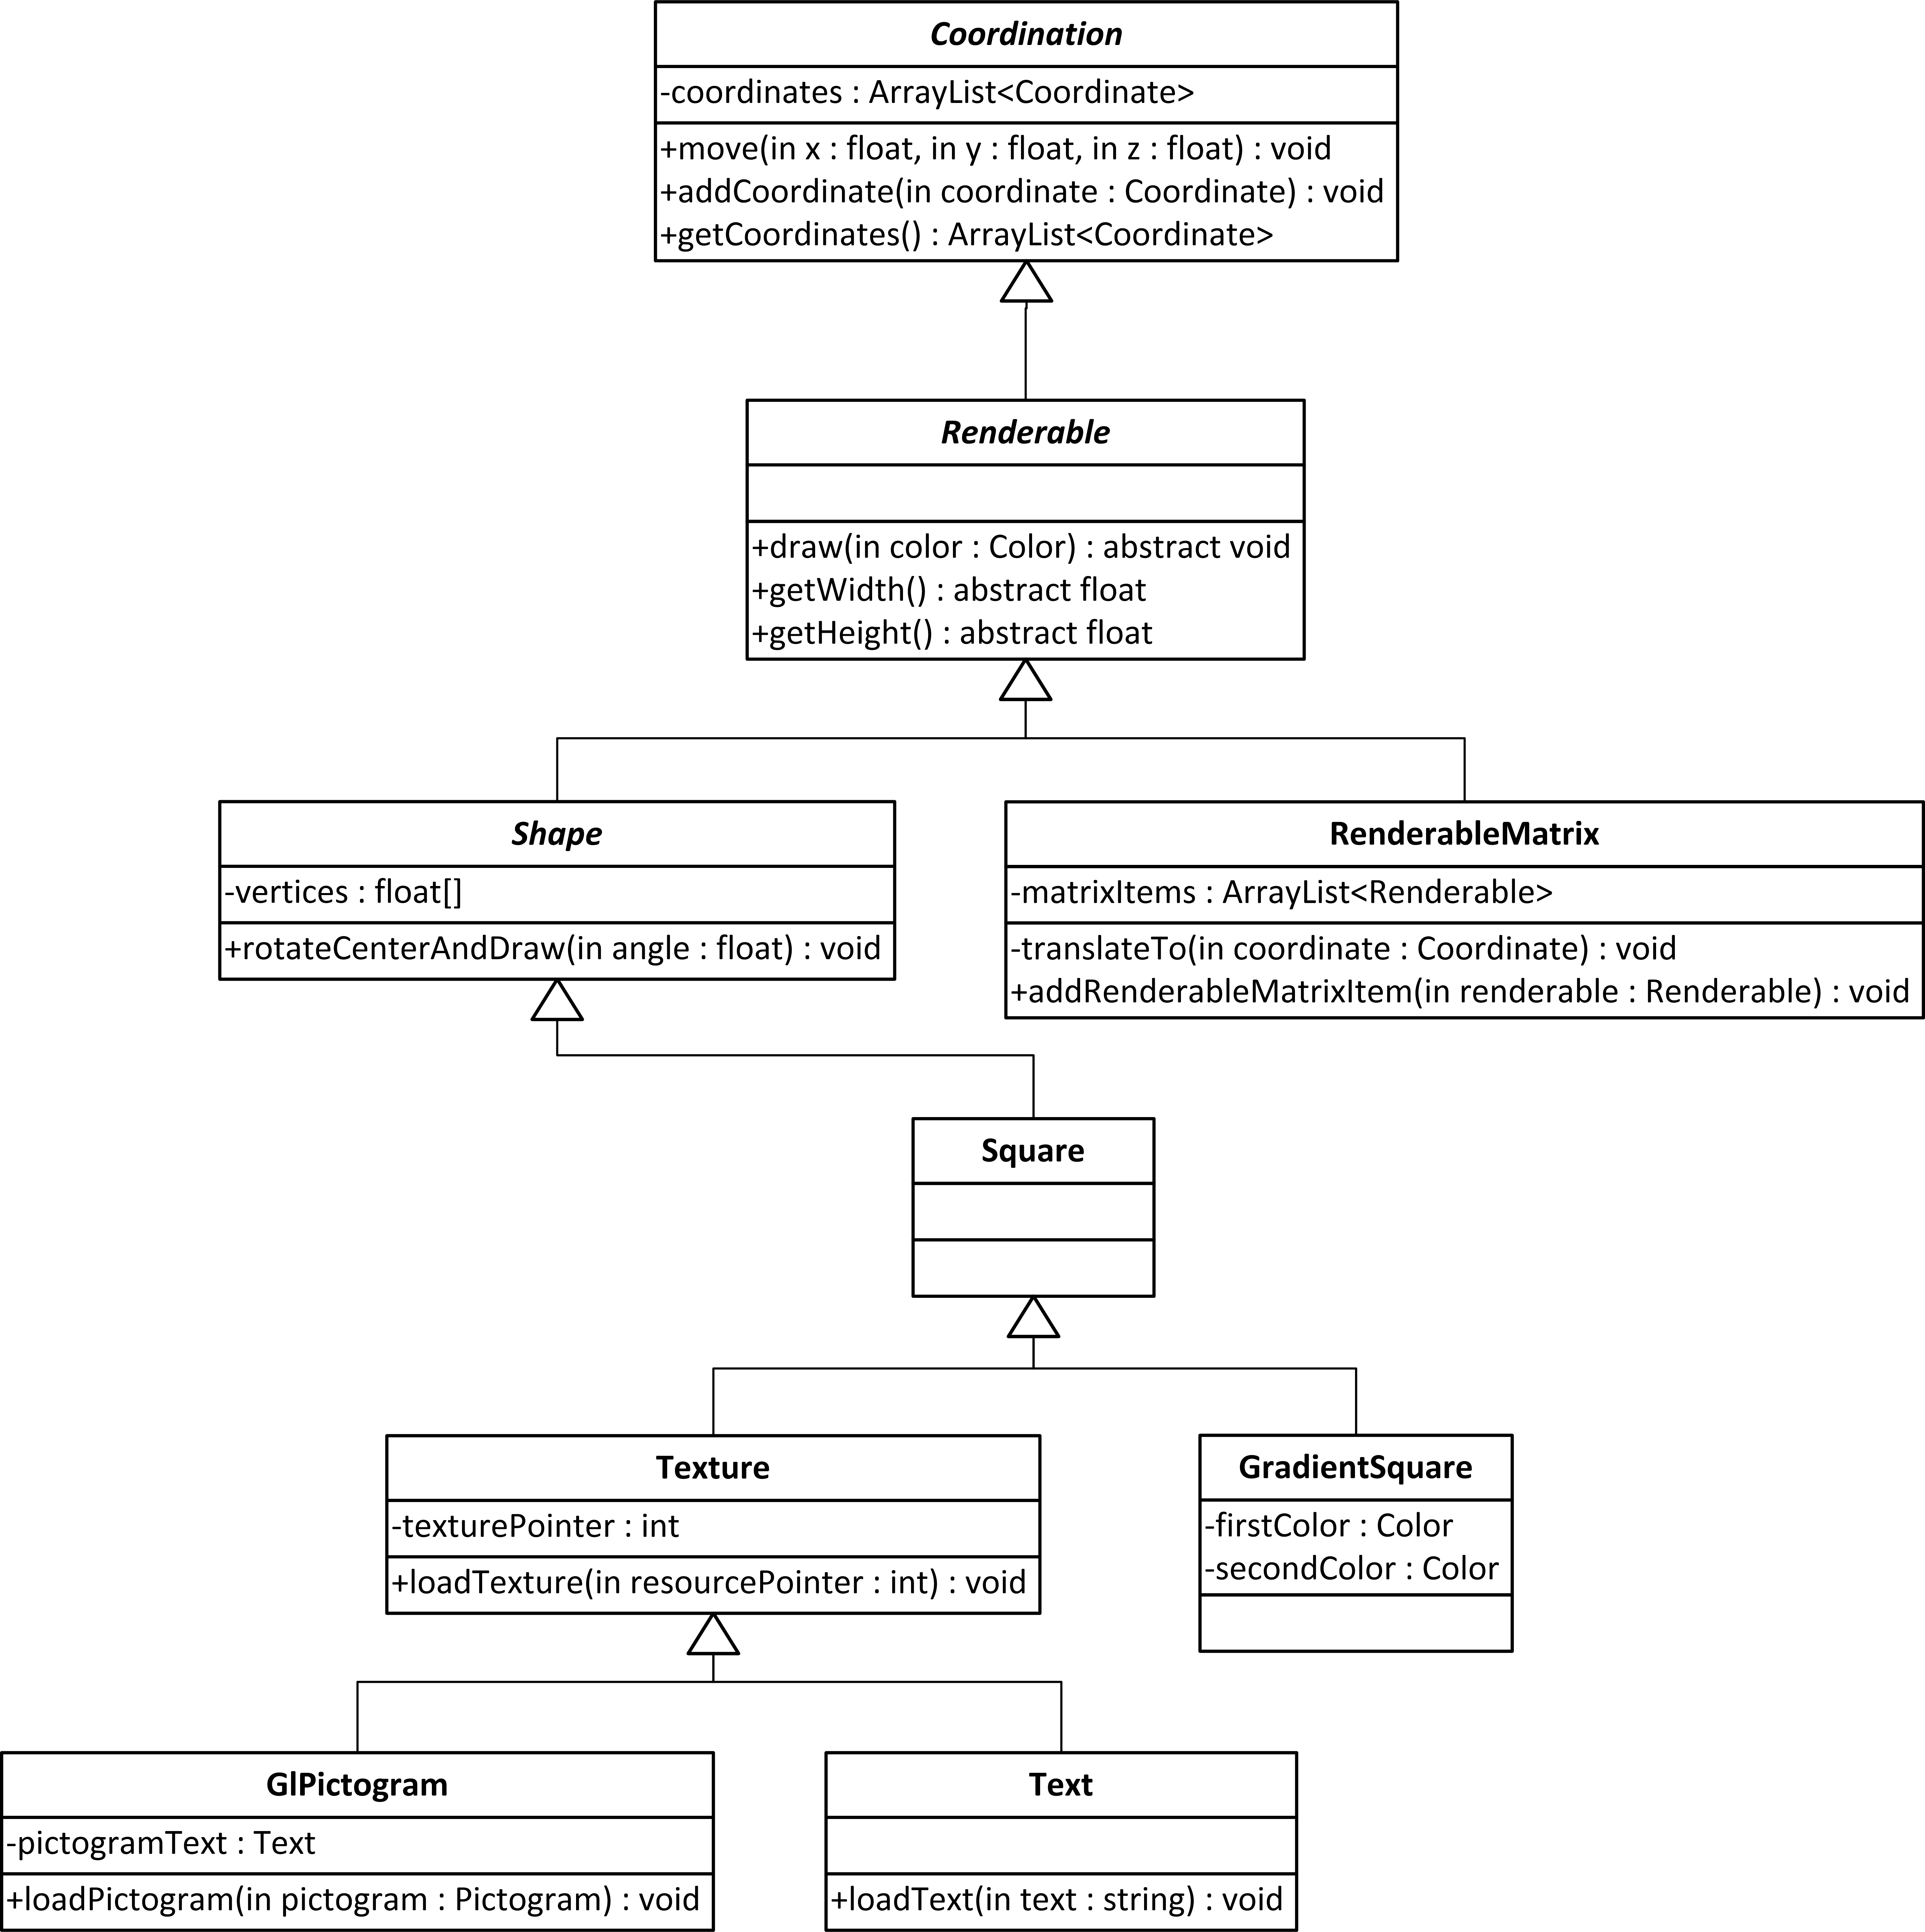
\includegraphics[width=0.9\linewidth]{img/renderables.png}%0.1 margin
\caption{Class diagram of the objects that can be rendered.}
\label{fig:renderables}
\end{figure}


\begin{figure}[H]
\centering
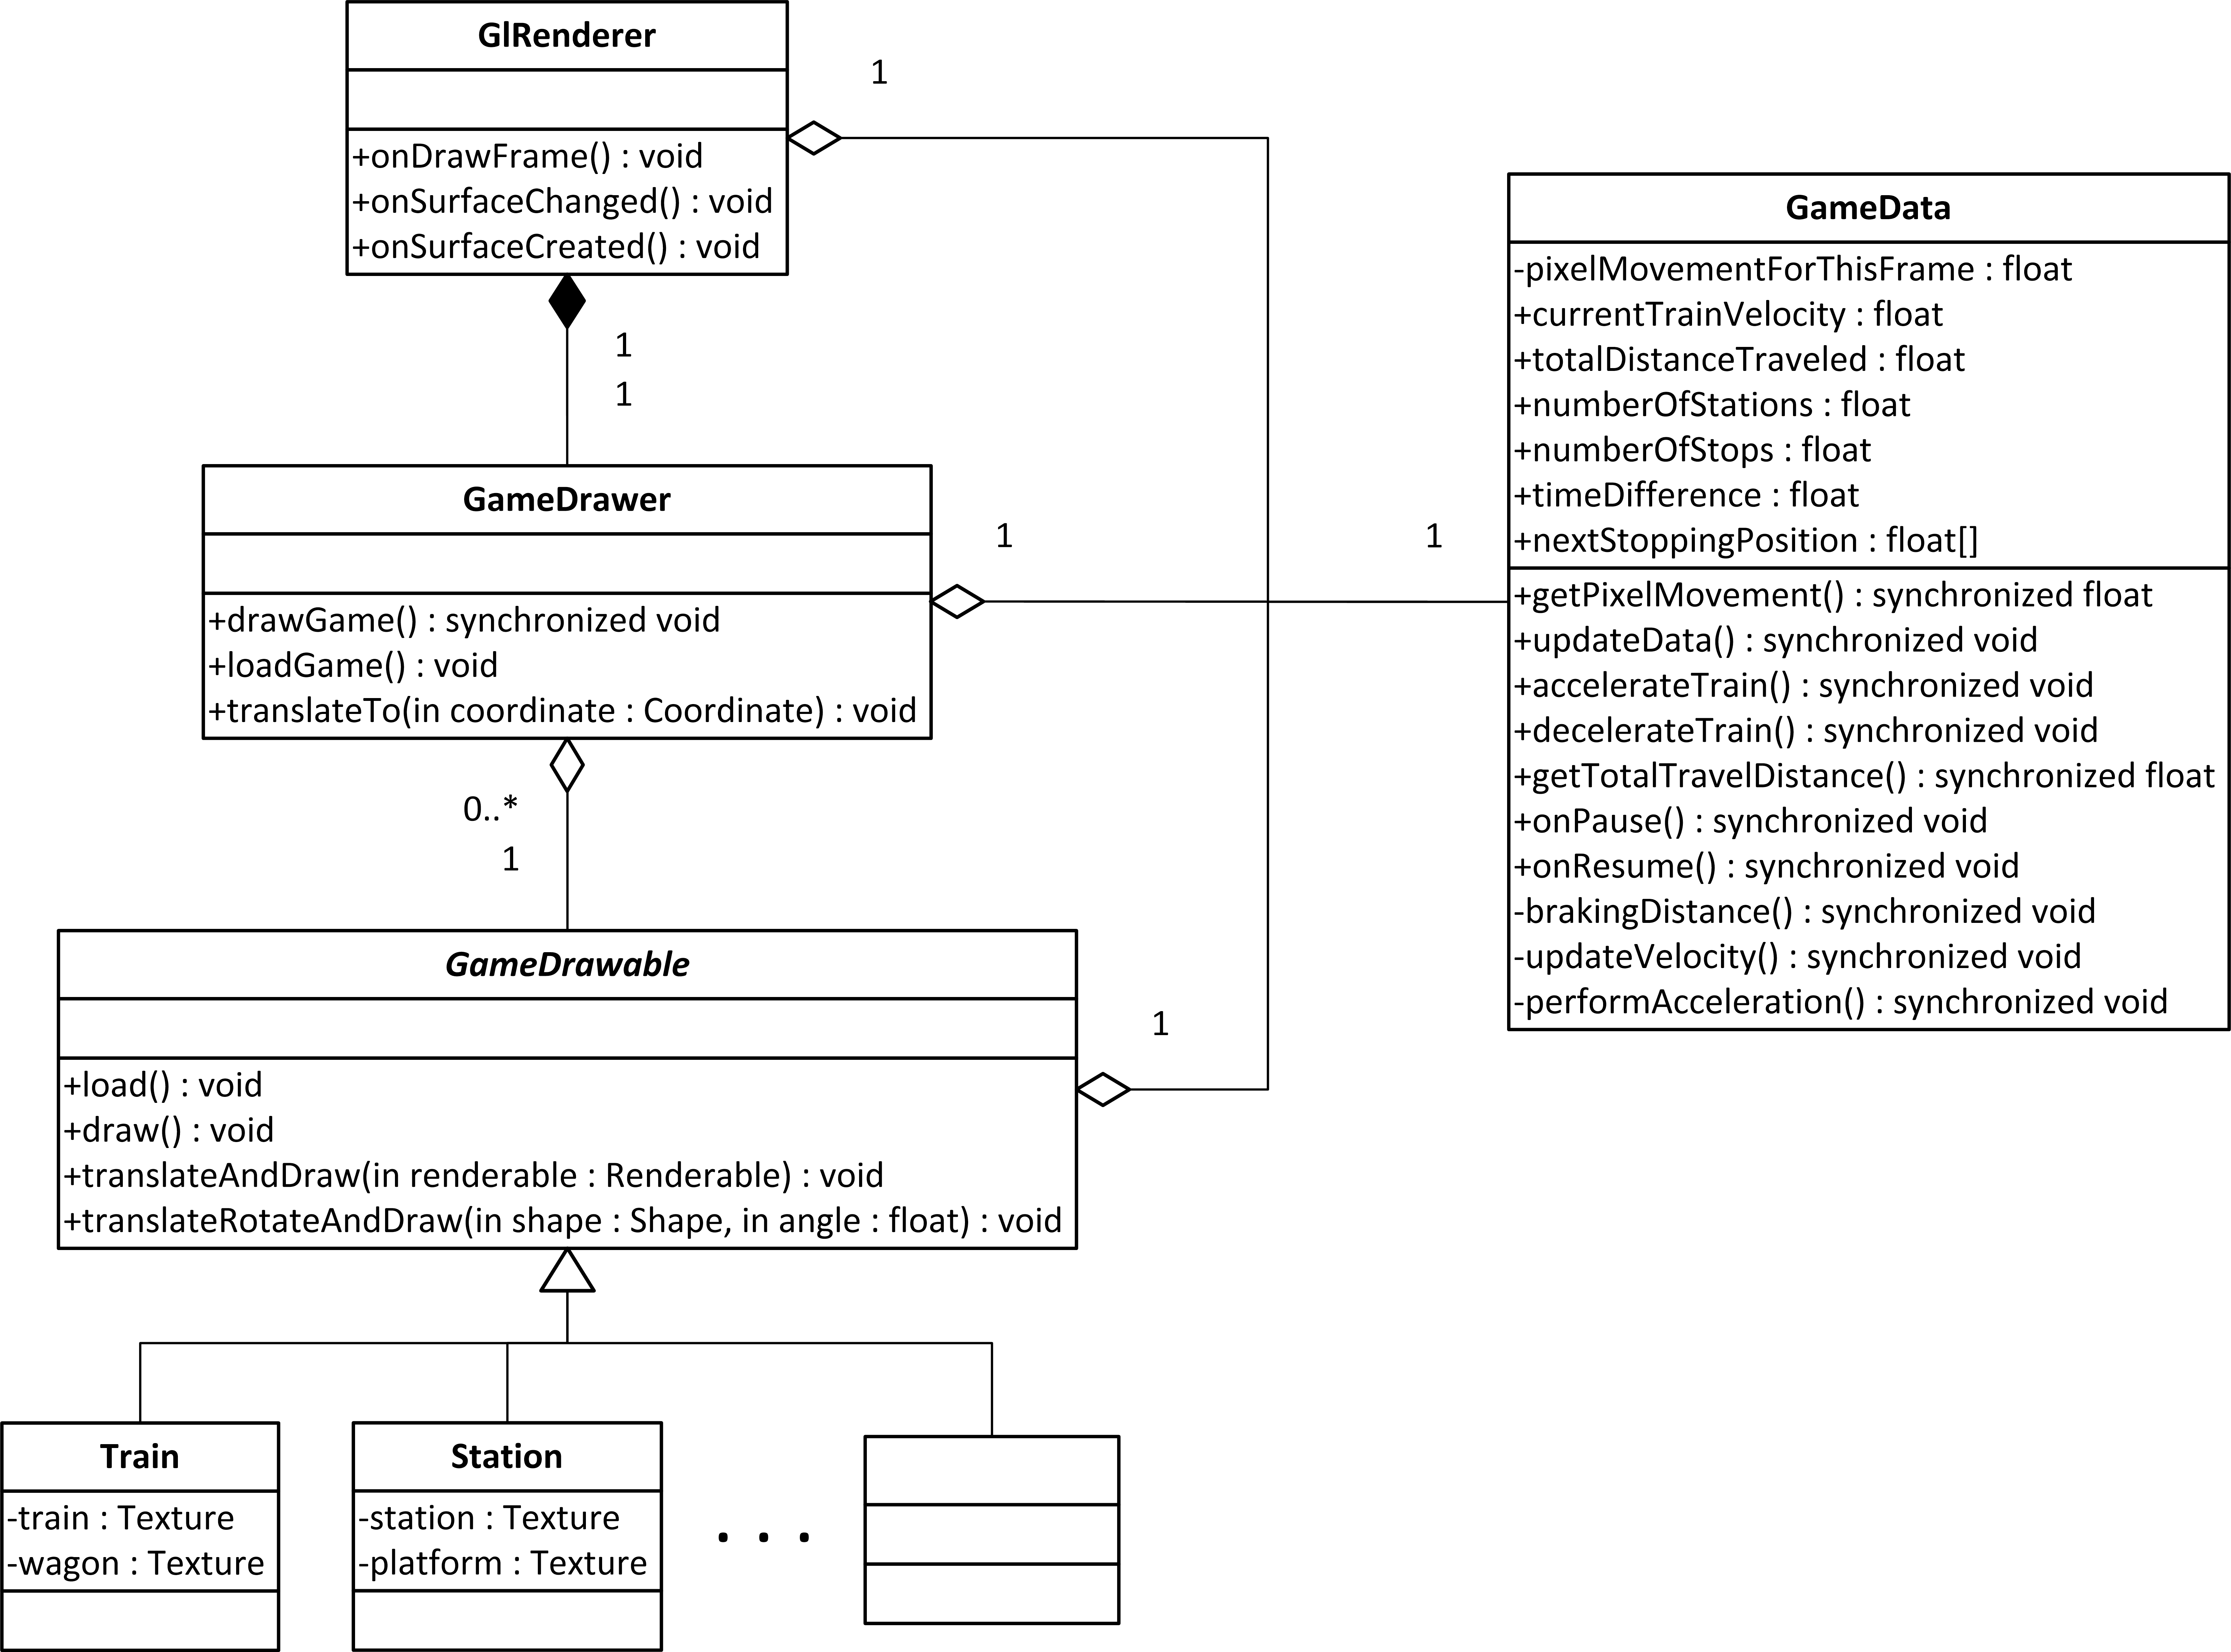
\includegraphics[width=0.9\linewidth]{img/game.png}%0.1 margin
\caption{Class diagram of the objects involved with drawing the game.}
\label{fig:game}
\end{figure}

\section{Implementation}

\todo{Describes the implementation of OpenGL}